\documentclass[9pt,twocolumn,twoside]{gsajnl}
% Use the documentclass option 'lineno' to view line numbers

\articletype{inv} % article type
% {inv} Investigation 
% {gs} Genomic Selection
% {goi} Genetics of Immunity 
% {gos} Genetics of Sex 
% {mp} Multiparental Populations

\title{Analysis of a The Cancer Genome Atlas (TCGA) RNA-seq data set on Uterine Corpus Endometrial Carcinoma (UCEC)}

\author[$\ast$]{Joaquim Aguirre}
\author[$\ast$]{Gerard Funosas}
\author[$\ast$]{Cristina Prat}

\affil[$\ast$]{University Pompeu Fabra}

\keywords{Uterine Corpus Endometrial Carcinoma; UCEC; TCGA; RNA-seq; Differential Expression; Functional Enrichment; Bioconductor}

\runningtitle{GENETICS | Investigation} % For use in the footer 

\correspondingauthor{Joaquim Aguirre}

\begin{abstract}
The Cancer Genome Atlas (TCGA) focuses on finding the genetic bases of cancer in human (\textit{Homo sapiens sapiens}) different tissues. The RNA sequencing tool provides information of the transcriptome of a biological sample in a given condition. Comparing tumorous and healthy samples, the differences in gene expression between those conditions can be uncovered. Uterine Corpus Endometrial Carcinoma (UCEC) is one of the most common cancers within women. In this study, a uterine RNA-seq dataset from TCGA has been analysed using bioinformatic tools. A paired sample sub-setting and a low-expressed genes filtering left a quality-filtered dataset of 11571 genes for 32 paired samples. After fitting the data in a regression linear model, taking into account both a surrogate variable analysis and one known covariate effect, the number of differentially expressed genes summed 7845 (68\%). The corresponding GO (Gene ontology) terms for each of those genes was assigned, and the most represented biological processes in the whole dataset were obtained and ordered by significance.  8 out of the 10 functional groups most differentially expressed in tumorous samples were related to cancer biochemical processes, such as tissue growth, immune response or cell signaling pathways. Another one was directly related to uterine muscle contraction, altered by cancer. Those results show that, even if the genetic bases of cancer are complex, there are both universal patterns in multiple kinds of cancer and specific ones for specific tumor types that can be further assessed to find new ways of controlling tumor development.
\end{abstract}

\setboolean{displaycopyright}{true}

\begin{document}

\maketitle
\thispagestyle{firststyle}
\marginmark
\firstpagefootnote
\correspondingauthoraffiliation{joaquim.aguirre01@estudiant.upf.edu}
\vspace{-11pt}%


\section*{Introduction}

Endometrial cancer develops in the cells that form the inner lining of the uterus, or the endometrium, and is one of the most common cancers of the female reproductive system. In 2010, approximately 43,000 women in the United States were estimated to have been diagnosed and almost 8,000 to have died of endometrial cancer. This cancer occurs most commonly in women aged 60 years or older. About 69 percent of endometrial cancers are diagnosed at an early stage, and as a result about 83 percent of women will survive five years following the time of diagnosis.

The Cancer Genome Atlas (TCGA) \citep{TheCancerGenomeAtlas} researchers have: 
\begin{itemize}
\item Identified four subtypes of endometrial cancer: POLE ultramutated, Microsatellite instability hypermutated, Copy number low and Copy number high.
\item Uncovered shared genomic features between endometrial cancer and serous ovarian cancer, the Basal-like subtype of breast cancer as well as colorectal cancer.
\item Identified three histologic diagnosis: Endometrioid endometrial adenocarcinoma, Mixed serous and endometrioid and Serous endometrial adenocarcinoma
\item Characterized the marked differences between the two types of endometrial tumors (endometrioid and serous), and found that some endometrioid tumors have developed a strikingly similar pattern to serous tumors, suggesting they may benefit from a common treatment.
\begin{itemize}
\item The serous and some of the endometrioid tumors are characterized by frequent mutations in TP53, extensive copy number alterations and few DNA methylation changes.
\item The rest of the endometrioid tumors are characterized by few copy number alterations, scarce mutations in TP53 and frequent mutations in PTEN and KRAS.
\end{itemize}
\end{itemize}

The comparison of transcriptional data between tumorous and healthy samples will revel gene expression differences specifically caused by the tumorous condition, and therefore will allow to find the main altered biochemical patters that cancer causes in the cells affected. That information may lead to further understanding of this illness and new possible treatments.
On that ground, the aim of the study is to find out which are the most significant biological pathways altered in tumorous cells of the uterine corpus. 

\section*{Materials and Methods}

The Bioconductor project \citep{Gentleman2004} is an open-source community effort to develop software packages on top of R for the analysis of molecular data obtained from high-throughput experimental technologies such as microarrays or high-throughput sequencing instruments.


\subsection*{Data Availability}
The SummarizedExperiment \citep{SummarizedExperiment} class was designed to meet requirements from high-throughput sequencing experiments such as storing molecular data from multiple assays and providing more flexibility to define the profiled features.

The RNA-seq data set on Uterine Corpus Endometrial Carcinoma (UCEC) have 20115 genes and 589 samples. Associated to the row (feature) data, there are 455 sequences (1 circular) from hg38 genome.

From the S4 object, it is possible to extract information about the gender of the patients who donated the samples, as well as other metadata. As the study is focused on endometrial cancer, all the samples must be from female patients, even if 33 of them showed 'NA' in the gender variable. Those were considered to be discarded from the beginning, but finally they were maintained as they provide the project with some normal (non tumorous) samples, which are not abundant in the dataset. Nevertheless, at last they were excluded by the paired filtering step. 

\subsection*{Quality assessment and normalization}
The fact that each RNA-seq sample may have been ultimately sequenced at slightly different depth and that there may be sample-specific bias related implies it may need to consider two normalization steps:
\begin{itemize}
\item Between-sample: adjustments to compare a feature across samples.
\begin{itemize}
\item Sample-specific normalization factors: using the TMM algorithm from the R/Bioconductor package edgeR \citep{Robinson2010b}.
\item Quantile normalization: using the CQN algorithm from the R/Bioconductor package cqn \citep{Hansen2012b}.
\end{itemize}
\item Within-sample: adjustments to compare across features in a sample.
\begin{itemize}
\item Scaling: using counts per million reads (CPM) mapped to the genome. This is already implemented in edgeR \citep{Robinson2010b} through the function cpm() which can take as input a DGEList object and can also output the CPM values in logarithmic scale.
\end{itemize}
\end{itemize}

It has been considered to discard those samples corresponding to the $ 10\% $ quartile of the sampledepth distribution, as the quality of the sequentiation of these samples is poorer. After that, the filtered set has 20115 genes and 527 samples.

It is important to work with a subset which is as much representative as the initial set of samples and that contains the samples with higher quality. The paired subsetting offers the advantage that as samples are paired, the posterior analysis of batch effect identification will be performed with a perfectly balanced set, which avoids confusions for not having samples of one of the variables. This step reduces the dataset to 36 paired samples.

The distribution of expression levels among samples and among genes in terms of logarithmic CPM units are checked. A cutoff of 1 unit of $log_{2}$ CPM is applied as minimum value of expression, in order to filter out lowly-expressed genes. The dataset ends up with 11571 genes.

The normalization factors are calculated on the filtered expression data set. The Trimmed Mean of M-values (TMM) method addresses the issue of the different RNA composition of the samples by estimating a scaling factor for each library. This is implemented in the edgeR package \citep{Robinson2010b} through the function calcNormFactors().

The MA-plots of the normalized expression profiles are performed. In general, there are not tumor samples with major expression-level dependent biases, although some of them show variations in low-expressed values. However, some normal samples show slightly expression-level dependent biases. The most suspicious cases are TCGA-AJ-A3NH, TCGA-AX-A2HC, TCGA-BK-A13C and TCGA-DI-A2QY, showing sizeable dependency between M and A values. 

\subsection*{Batch effect identification and removal}

Tissue Source Site (TSS) is used as surrogate of batch effect indicator variable. It is examined how samples group together by hierarchical clustering and multidimensional scaling by Spearman correlation, annotating the outcome of interest and the surrogate of batch indicator.

In the multidimensional plot (MDS) and the hierarchical clustering it is shown that TCGA.AX.A2HC.01A and TCGA.DI.A2QY.11A samples are problematic as was seen in the MA-plots. Therefore, both samples and their paired ones are removed. The final dataset ends up with 32 samples and 11571 genes.

Moreover, the sva \citep{sva} R/Bioconductor package provides a function called ComBat(), an empirical Bayes method robust to outliers in small sample sizes which removes batch effect. ComBat is used in the dataset to remove variability that is not related with the conditions studied.

\subsection*{Differential expression}

We perform a simple examination of expression changes and their associated p-values using the R/Bioconductor package SVA \citep{sva}. Surrogate variable analysis (sva) is a technique that tries to capture sources of heterogeneity in high-throughput profiling data, such as non-biological variability introduced by batch effects. The output of SVA is an estimation of the number of so-called “surrogate variables” and their continuous values, which can be used later on to adjust for these unmeasured and unwanted effects.The SVA algorithm are used to assess the extent of differential expression this time adjusting for these surrogate variables.  

\begin{table} 
\centering
\caption{Linear regression models created and their corresponding number of differentially expressed genes found}
\begin{tableminipage}{\textwidth}
\begin{tabular}{c c c} 
\hline
Model & Approach used & DE genes \\ [0.5ex]
\hline
1 & Fit directly the linear model & 6457 \\
2 & Adjust for mean-variance relationship & 6441 \\
3 & Adjust for known covariates & 6491 \\
4 & Adjust for known covariates + SVA & 7845 \\
\hline
\end{tabular}
  \label{tab:model_go}
\end{tableminipage}
\end{table}

After that, different types of linear regression models are built in order to assess differential expression. The conceptual purpose of a linear regression model is to represent, as accurately as possible, something complex, the data denoted by y, which is n-dimensional, in terms of something much simpler, the model, which is p -dimensional. Thus, if the model is successful, the structure in the data should be captured in those p dimensions, leaving just random variation in the residuals which lie in an (n-p)-dimensional space. In the context of DE analysis, linear regression models can be written in matrix form, design matrices. The design matrix contains as many rows as samples and as many columns as coefficients to be estimated. The limma \citep{Ritchie2015} R/Bioconductor package has been used to calculate DE analysis.

If the outcome of interest is not confounded with other sources of variation, the more variables there are in the linear model, the fewer degrees of freedom it has, and therefore the less statistical power it shows.

\subsection*{Functional enrichment}

Functional enrichment analyses constitute a straightforward way to approach the question of what pathways may be differentially expressed (DE) between normal and tumor genes in our data.

The Gene Ontology (GO) database project provides a controlled vocabulary to describe gene and gene product attributes in any organism. It consists of so-called GO terms, which are pairs of term identifier (GO ID) and description. The GOstats \citep{Falcon2007} R/Bioconductor package performes a functional enrichment analysis on the entire collection of GO gene sets. A parameter object with information specifiying the gene universe, the set of DE genes and the annotation packages org.Hs.eg.db \citep{org.Hs.eg.db} to use are built. The functional enrichment analysis is turned by a conditional test which takes into account the hierarchical structure of GO terms.


\section*{Results and Discussion}

\subsection*{Quality assessment, normalization, Batch effect identification and removal}

A better stratification of the tumor and normal samples are shown when ComBat is applied (Figure \ref{fig:Hierarchical clustering}). The chosen factor whose variability has been removed is the TSS (differences depending on the tissue source site).

\begin{figure}[htbp]
\centering
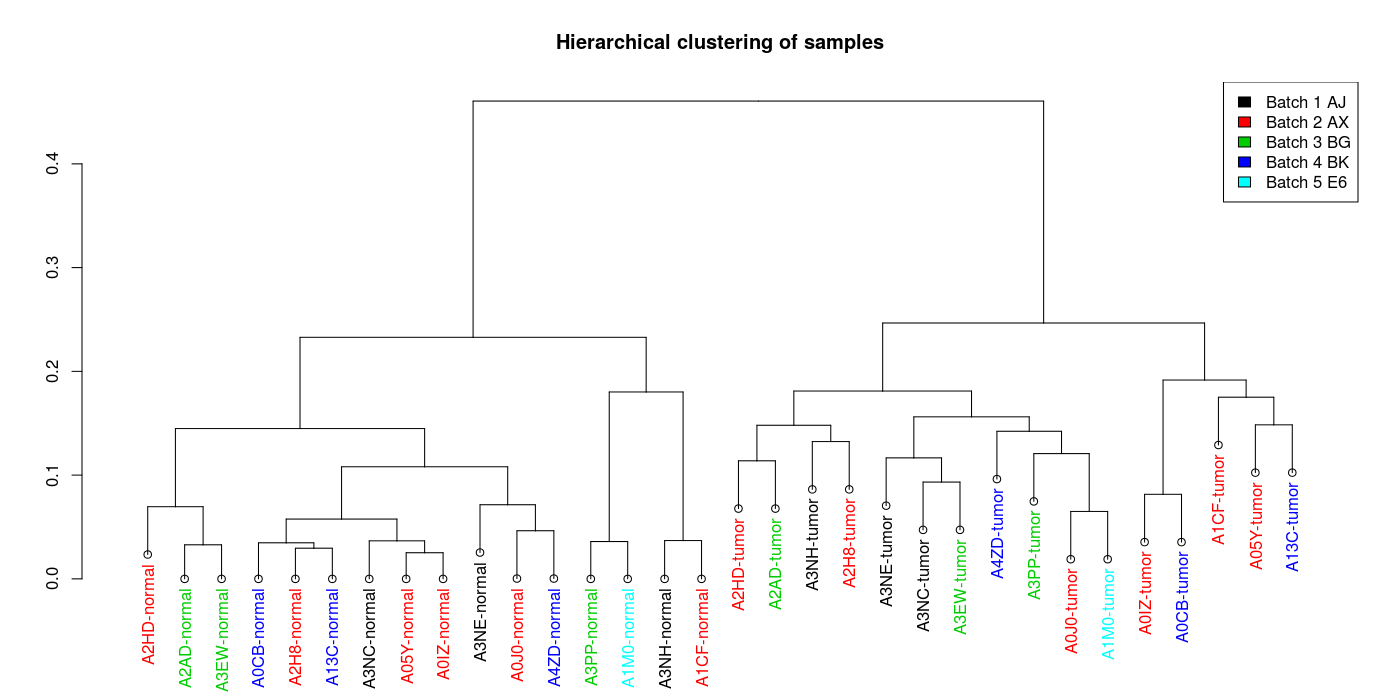
\includegraphics[width=\linewidth]{sampleClustering_3-1}
\caption{Hierarchical clustering of the samples with the TSS batch effect removed}
\label{fig:Hierarchical clustering}
\end{figure}

\subsection*{Differential expression analysis}

From the differential expression analysis, four different models were created in order to assess differential expression (Table \ref{tab:model_go}), all of them using a False Discovery Rate (FDR) of 5\%. The first was the simplest one, as the linear model was fitted directly in the design matrix to every gene. 6457 genes were differentially expressed using this approach. The second model consisted in fitting the model adjusting for the mean-variance relationship. This is done in order to correct the variability of RNA-seq counts from sample to sample for the same gene and different depths of different samples. The results obtained were 6441 differentially expressed genes. The third model was adjusting the model for known covariates, known sources of unwanted variation. The source of variation used was the TSS, obtained from the patient barcode. The results were 6491 differentially expressed genes. The fourth analysis was to complement the previous model of known covariates with a surrogate variable analysis (SVA). There were 9 surrogate variables found, which were added to the design matrix of the third model. The MA-plot corresponding to the fourth model is represented in Figure \ref{fig:MAplot}. From this analysis, 7845 differentially expressed genes were found. In all the models created the chromosome with higher number of differentially expressed genes was the chromosome 1.

\begin{figure}[htbp]
\centering
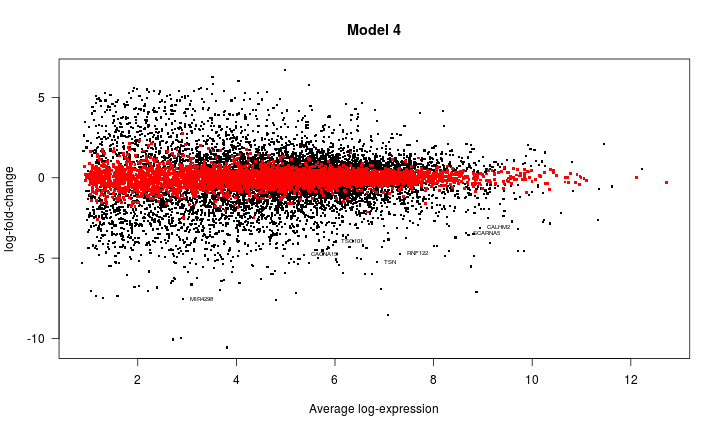
\includegraphics[width=\linewidth]{maPlot-1}
\caption{MA-plot for the model 4, adjusting the known covariate TSS and unkwnown covariates using SVA}
\label{fig:MAplot}
\end{figure}

The more complete linear model is the last one, as it includes to an adjusted model for mean-variance relationship the adjustment to variability of known and unknown covariates. The number of differentially expressed genes increases importantly in this model with respect to the others, which means that has more statistical power. If that happens with a model that takes into account more variables (and therefore has fewer degrees of freedom) it is because the model has been adjusted for the data heterogenity that was difficulting the statistical power. Therefore, the model that is going to be used for posterior Functional Enrichment Analysis is the fourth model, adjusting for known covariates plus the SVA.

From this last linear model, a factorial design was performed in order to analyse the interaction between type (tumor or normal) and TSS, concretely with BG and BK. It was not successful, as there were not genes which were clearly differentially expressed in only one of them. For future analyses, it could be interesting to analyse the interaction between other possible sources of unwanted variation such as histological diagnosis, as it has been seen in several studies that there are genes clearly differentially expressed between serous and endometroid tumors \citep{Getz2013}.



\subsection*{Functional Enrichment}

Table \ref{tab:shape-functions} shows the list of the 10 most significantly differentially expressed pathways in uterine tumour tissue, taking the ordered goresults obtained from the final set of DEgenes. 

\begin{table}
\centering
\caption{Ten most significant gene ontologies found in the Functional Enrichment analysis}
\begin{tableminipage}{\textwidth}
 \begin{tabular}{| c c c c c |} 
 \hline
 \textbf{GOBPID} & \textbf{Pvalue} & \textbf{OddsRatio} & \textbf{Excount} & \textbf{Count} \\ [0.5ex] 
 \hline
 GO:0010762 & 0.0068 & Inf & 8.8567 & 13 \\
 \multicolumn{5}{|c|}{regulation of fibroblast migration} \\ 
 \hline
 GO:1903543 & 0.0100 & Inf & 8.1754 & 12 \\ 
 \multicolumn{5}{|c|}{positive regulation of exosomal secretion} \\ 
 \hline
 GO:0007213 & 0.0146 & Inf & 7.4941 & 11 \\
 \multicolumn{5}{|c|}{G-protein coupled acetylcholine receptor signaling pathway} \\ 
 \hline
 GO:0032735 & 0.0146 & Inf & 7.4941 & 11 \\
 \multicolumn{5}{|c|}{positive regulation of interleukin-12 production} \\ 
  \hline
 GO:0046636 & 0.0146 & Inf & 7.4941 & 11 \\ 
 \multicolumn{5}{|c|}{negative regulation of alpha-beta T cell activation} \\ 
  \hline
 GO:0071380 & 0.0146 & Inf & 7.4941 & 11 \\
 \multicolumn{5}{|c|}{cellular response to prostaglandin E stimulus} \\ 
  \hline
 GO:0010842 & 0.0215 & Inf & 6.8128 & 10 \\
 \multicolumn{5}{|c|}{retina layer formation} \\ 
  \hline
 GO:0036092 & 0.0215 & Inf & 6.8128 & 10 \\
 \multicolumn{5}{|c|}{phosphatidylinositol-3-phosphate biosynthetic process} \\ 
  \hline
 GO:0045986 & 0.0215 & Inf & 6.8128 & 10 \\
 \multicolumn{5}{|c|}{negative regulation of smooth muscle contraction} \\ 
  \hline
 GO:0007063 &  0.0316 & Inf & 6.1316 & 9 \\
 \multicolumn{5}{|c|}{regulation of sister chromatid cohesion} \\ 
 \hline
\end{tabular}
\label{tab:shape-functions}
\end{tableminipage}
\end{table}

Taking those 10 top GO terms, nine functional groups are identified  which could be, directly or indirectly, involved in endometrial cancer. One of them seems to be a functional group specific from our cancer type, while the others do not. Another one, related to the retina formation, does not seem to be biochemically related to the UCEC. 

Between the eight groups that can be related to cancer:
\begin{itemize}
  \item Regulation of fibroblast migration, which is directly related with tissue damage, and therefore, with tumors. Fibroblasts are considered to have a key role in the malignant progression of cancer and represent an important target in endometrial cancer research, as it has been demonstrated in some previous articles \citep{Subramaniam2013, Teng2016, Turner2010}.
  \item Regulation of sister chromatid cohesion, as it has been proved that aberrant sister chromatid cohesion causes instability and contributes to the development of cancer \citep{LeGallo2012}. Several studies have targeted candidate chromosome instability genes in order to treat endometrial cancer \citep{Price2013}.
  \item Positive regulation of exosomal secretion, which is fundamental due to the increasing evidence that tumor cells release excessive amount of exosomes \citep{Zhang2015}.
  \item Regulation of interleukin-12 production and alpha-beta T cell activation are clearly part of the development of the immune response against the tumor \citep{Colombo2002, Martin-Orozco2009}, and therefore, they are differentially expressed in comparison with normal samples. 
  \item G-protein coupled receptor pathway or phosphatidyli-nositol-3-phosphate biosyntesis are two cases belonging to signaling pathways, also affected by cancer development \citep{Li2005, Wang2006}.
\end{itemize}

There is one group identified between the top ten differentially expressed functional groups which has been directly related with endometrial cancer: negative regulation of smooth muscle contraction. This is because fibroids, which are benign tumours of smooth muscle, are believed to alter muscular contraction of uterus \citep{GeorgetownUniversityHospital}. However, there is not much investigation in this direction.

It is also important to remark that there are two differentially expressed genes known to have important roles in endometrial cancer which are part of two of the top ten differentially expressed functional groups. The first is PIK3C2A, which is part of the Phosphatidylinositol-3-phosphate biosynthetic process, and has an established role in the pathogenesis of serous endometrial cancer \citep{LeGallo2012}. The second is CTNNB1, in regulation of sister chromatid cohesion, a gene with an unusually high frequency of mutations in endometroid tumors (52\%) \citep{Getz2013}.

The differential expression and functional enrichment analysis have provided an interesting perspective of the endometrial cancer, remarking the most important genes and pathways which suffer changes during the disease, and raising hypotheses about how they could affect to its advance. 

\subsection*{Conclusions} 

The main source of variation of the dataset seems to be driven by the tumor and normal condition of the samples, as seen in the Figure \ref{fig:Hierarchical clustering}. The hierarchical clustering of the samples showed a better stratification when adjusting for the tss factor, without this batch effect. 

The SVA analysis helps identifying more differentially expressed genes, since ajusting for other sources of variation leads to more statistical power in the model and hence to more DE genes found. 

The functional enrichment analysis with GO terms identified nine out of the ten most differentially expressed groups that perfectly fit in the pattern of a tumorous development. 

One of those nine cancer related GO terms, defined as negative regulation of smooth muscle contraction, can be specifically related to the endometrial cancer. 

At least two found differentially expressed genes (PIK3C2A, CTNNB1) are known to be involved specifically to endometrial cancer. 

\section*{Acknowledgments}

We thank Juan Roberto Castelo Valdueza for various encouraging discussions on this work. Also we thank The Cancer Genome Atlas (TCGA) which provide the studying data .

\bibliography{IEO_UCEC}

\end{document}